\chapter{ISTTOK }

\section{Machine description}


\begin{figure}[htbp]
	\centering
	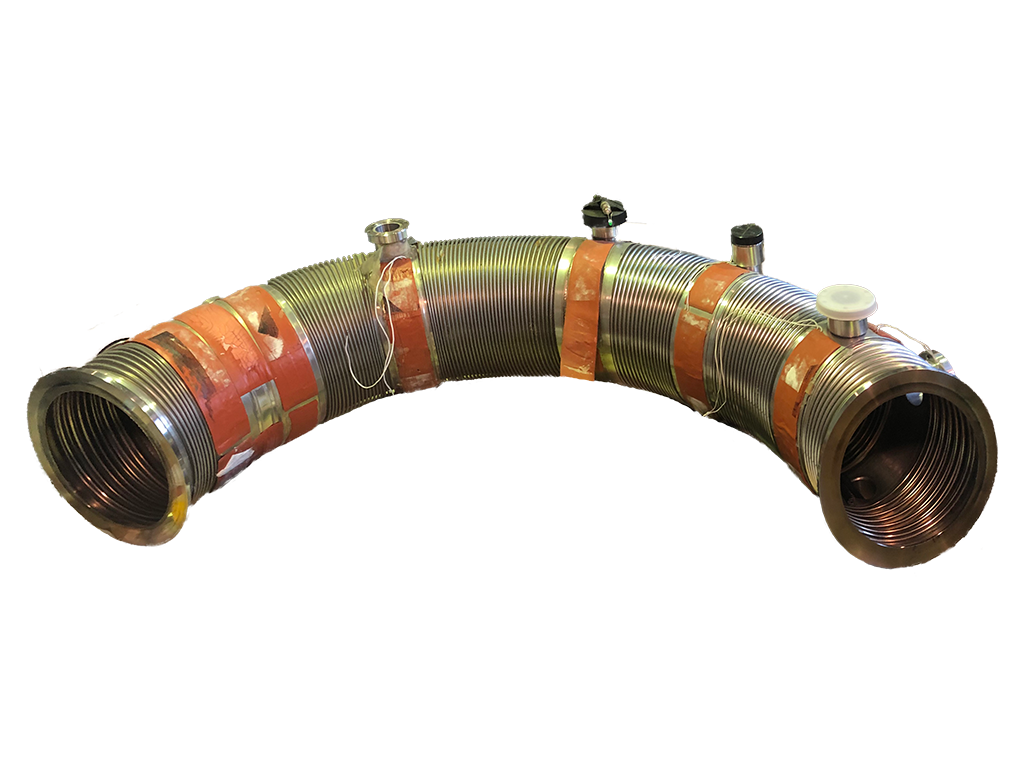
\includegraphics[width=0.65\textwidth]{Chp4/VacuumVessel_Low.png}
	\caption{\label{VV_IST} Actual ISTTOK vaccum vessel section with ports.  }
\end{figure}


\begin{figure}[htbp]
	\centering
	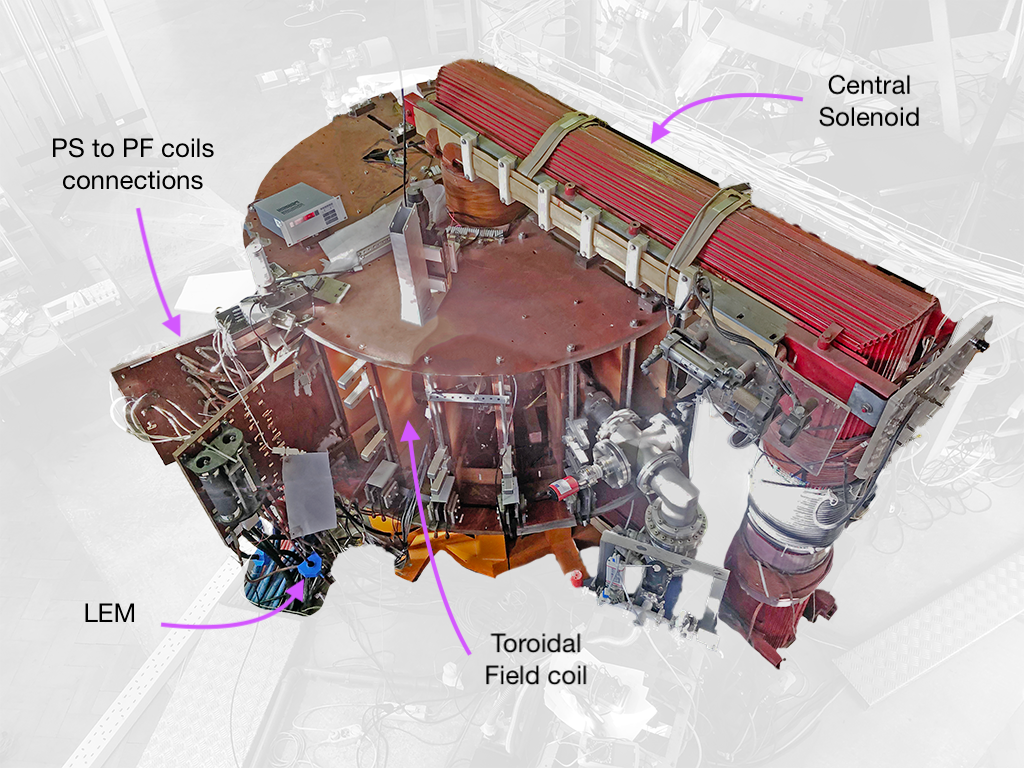
\includegraphics[width=0.95\textwidth]{Chp4/TopISTTOK.png}
	\caption{\label{TopISTTOK} ISTTOK top view in 2020,   main elements are indicated with magenta  lines.}
\end{figure}

\begin{figure}[htbp]
	\centering
	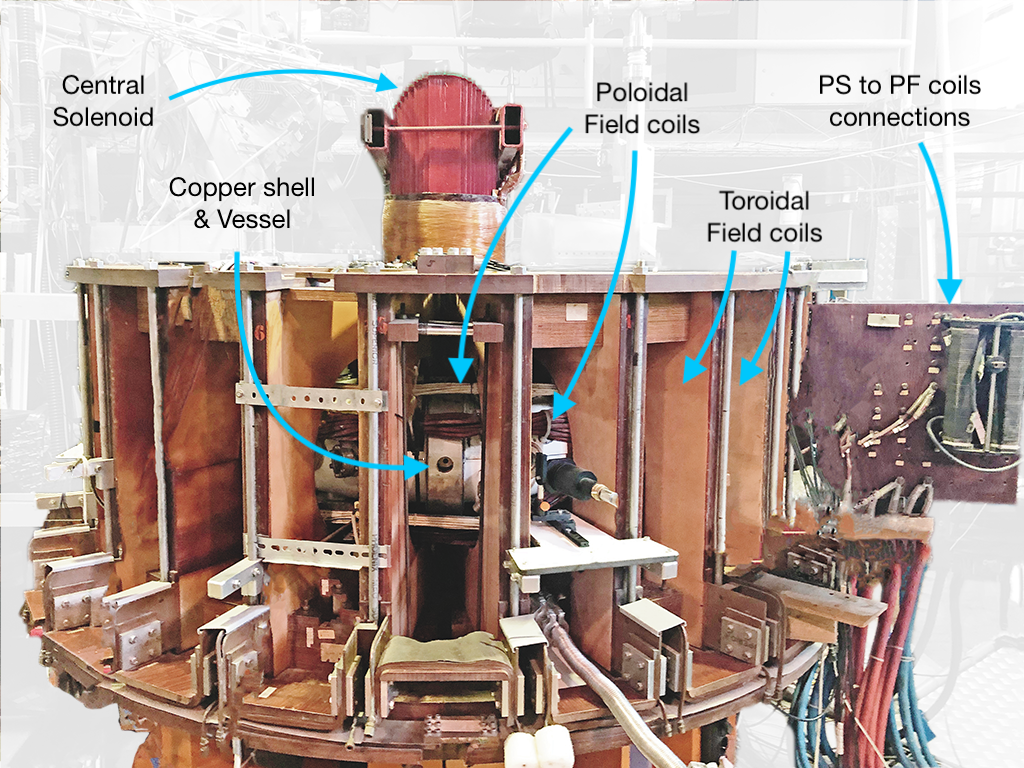
\includegraphics[width=0.95\textwidth]{Chp4/FrontISTTOK.png}
	\caption{\label{ISTTOK_front}ISTTOK frontal view in 2020, main elements are indicated with blue lines.   }
\end{figure}




\section{Diagnostics and Actuators}

\begin{figure}[htbp]
	\centering
	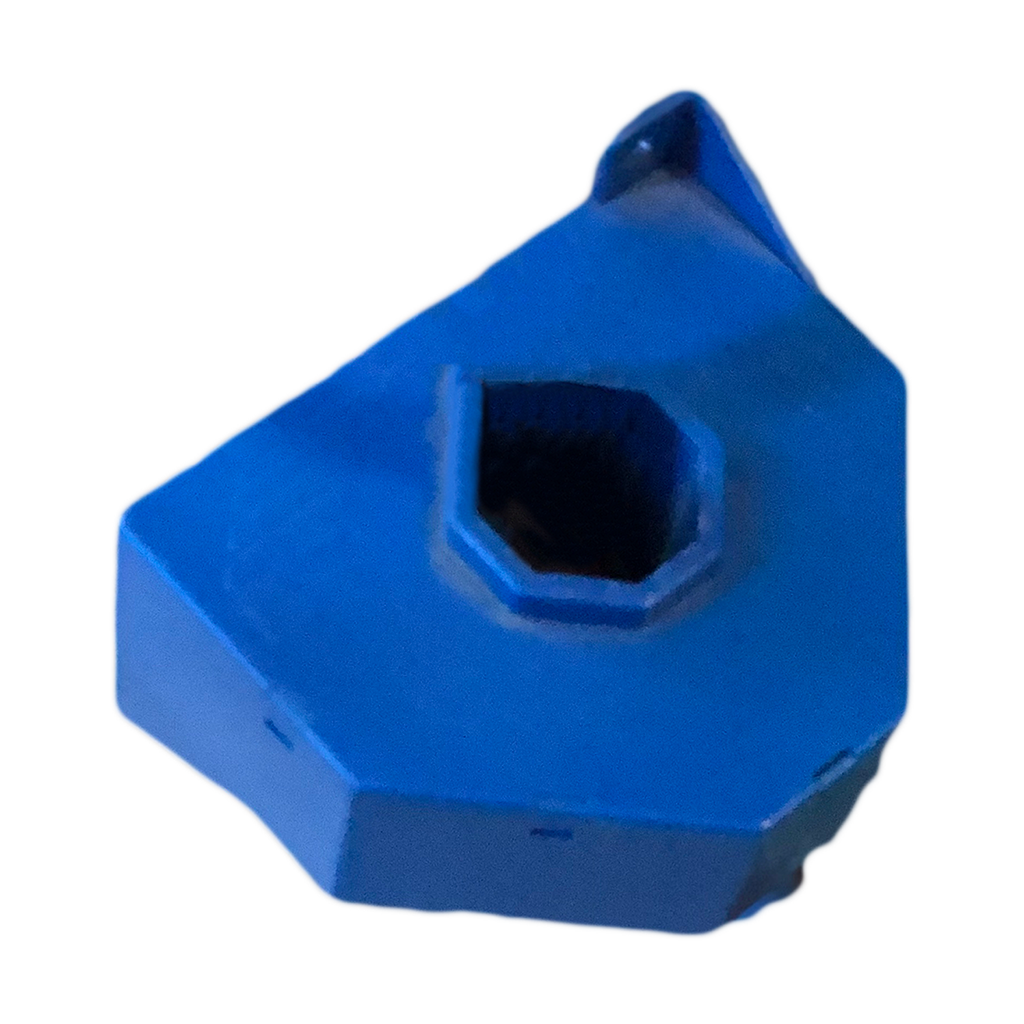
\includegraphics[width=0.4\textwidth]{Chp4/LEM.png}
	\caption{\label{LEM} LEM }
\end{figure}

\begin{figure}
	\centering
	\begin{subfigure}[b]{0.37\textwidth}
		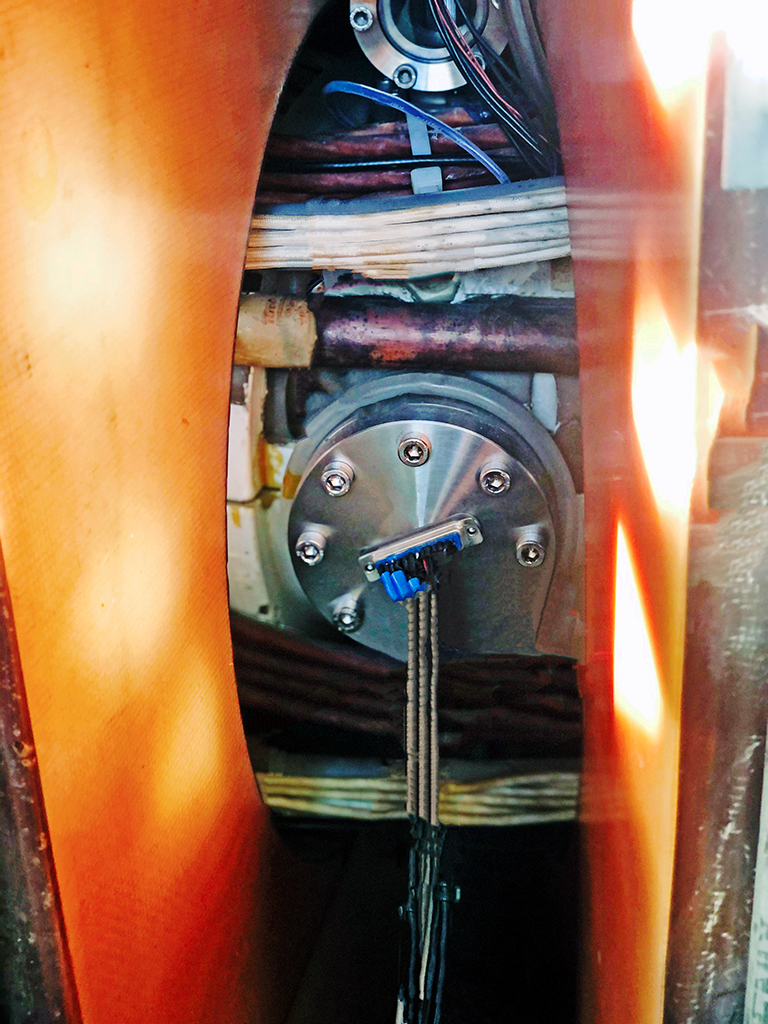
\includegraphics[width=\textwidth]{Chp4/PuertoMirnov.png}
	\caption{\label{MirnPort}Magnetic probes port whith connection cable to the ATCA adquisition boards, also PF coils and cooper shell are shown. }
	\end{subfigure}
~~~~
	\begin{subfigure}[b]{0.37\textwidth}
		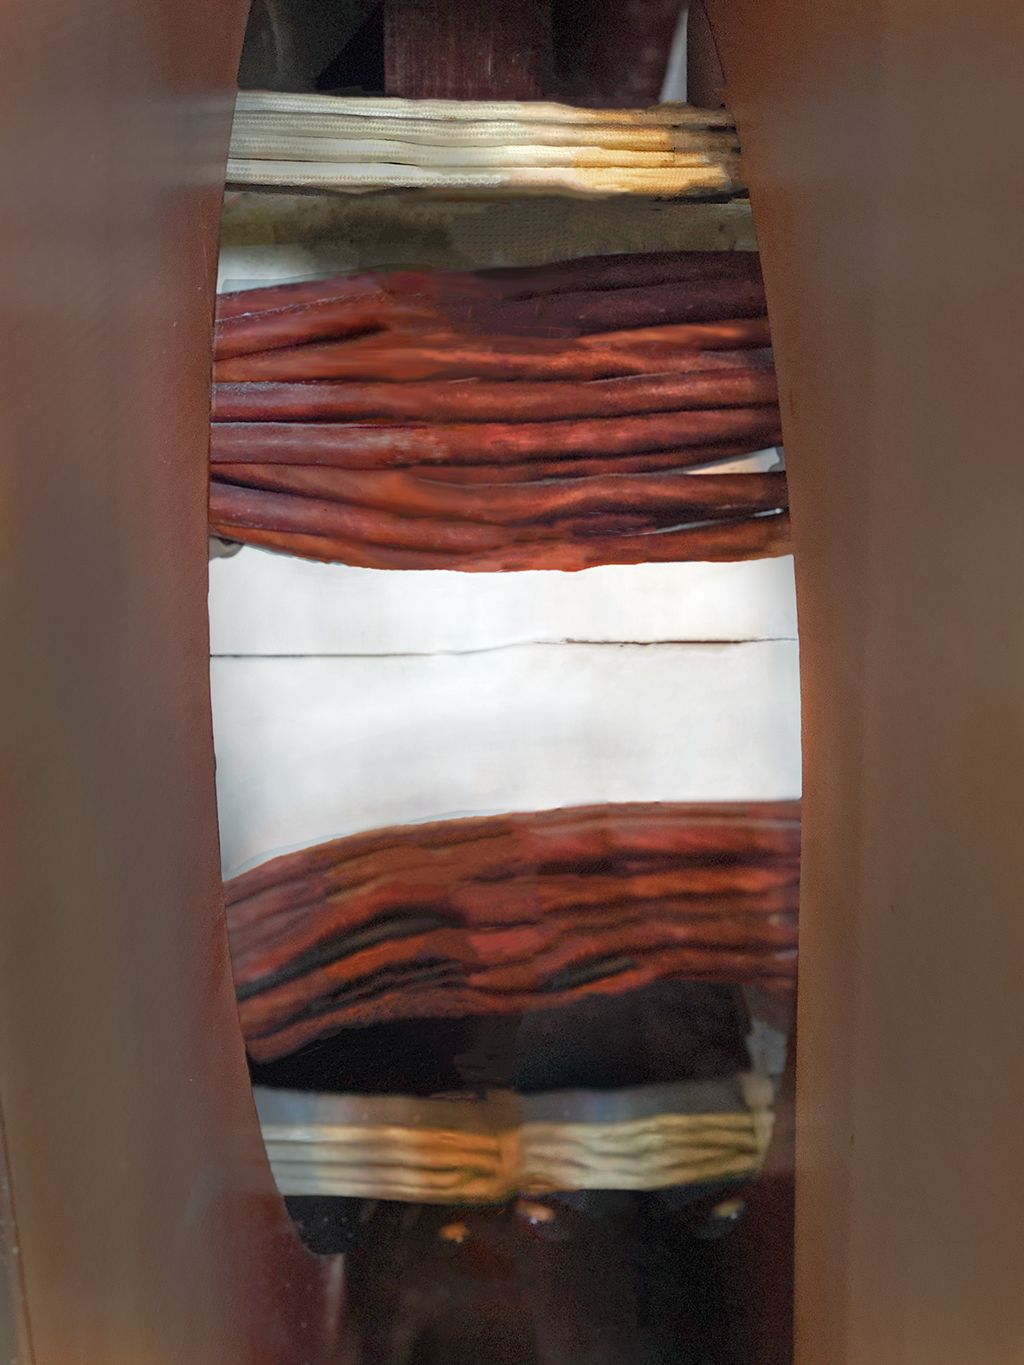
\includegraphics[width=\textwidth]{Chp4/PFCoils.png}
	\caption{\label{ISTTOKpfCoils}PF coils close up,primary coils correspond to the  white cables and vertical and horizontal to the orange ones. }
\end{subfigure}

 \caption{ISTTOK close up side views. \label{ISTTOKviews} }
\end{figure}




\section{ATCA-MIMO-ISOL boards}
\subsection{Hardware layout}
\subsection{Real-time  integration software}
\section{Plasma current magnetic field }

Retrieving the contribution of the plasma current in tokamaks ...

The methods of correction of the magnetic error fields due to inaccuracies
of tokamak manufacturing and assembly are considered. The problems of the
plasma position and shape reconstruction based on magnetic field measurements are discussed.

\section{Plasma centroid position determination}